\documentclass[a4paper,11pt]{article}
\usepackage{latexsym}
\usepackage[utf8]{inputenc}
\usepackage[activeacute,spanish]{babel}
\usepackage{lineno}
\RequirePackage{graphicx}
\RequirePackage{booktabs}

\usepackage[colorlinks,linkcolor={blue},citecolor={blue},urlcolor={red}]{hyperref}
\hypersetup{urlcolor=blue, colorlinks=true} % Colors hyperlinks in blue

\linespread{1.2} % Interlineado
\usepackage{geometry} % Control de margenes
 \geometry{
 left=24mm,
 right=24mm,
 top=24mm,
 bottom=24mm
 }

%opening
\title{Formato Básico de Artículo de Investigación}
\author{César Jiménez \\
 Universidad Nacional Mayor de San Marcos \\
\emph{cjimenezt@unmsm.edu.pe}\\}

\begin{document}
%\linenumbers % Coloca numeracion a las lineas
\maketitle

\begin{abstract} \noindent 
Aqui va el Resumen del trabajo de investigación. Este formato en Latex puede ser utilizado durante el proceso de revisión por pares.\\
\textbf{Palabras clave}: clave1, clave2, clave3.
\end{abstract}

\centerline{\textbf{Basic Format of Research Paper}} 
\renewcommand{\abstractname}{Abstract}

\begin{abstract} \noindent		
Here is the Abstract of the research. This format in Latex can be used in the peer review process.\\
\textbf{Keywords}: key1, key2, key3.
\end{abstract}


\section{Introducción}
Esto es la introduccion. Las citaciones se realizan de esta manera: \cite{1}. Las referencias se colocan de acuerdo al orden de aparición de las citaciones \cite{2}, de acuerdo al formato APS \cite{3}.

\begin{equation}
F_e = k \frac{q_1 q_{2}}{r^2} 
\end{equation}

\subsection*{Área de estudio}

\subsection*{Antecedentes}

\section{Datos}
Ejemplo de ecuacion:
\begin{equation}
\label{1}
\ {s(t)} = u(t)*f(Q,t)*I(t) \
\end{equation}

\section{Metodología}
Ejemplo de ecuacion larga:
\begin{eqnarray}
\label{2}
\frac{\partial M}{\partial t}+\frac{\partial}{\partial x}\left(\frac{M^2}{D}\right)+\frac{\partial}{\partial x}\left(\frac{MN}{D}\right)=-gD\frac{\partial\eta}{\partial x} \nonumber\\
-\frac{gn^2}{D^{7/3}}M\sqrt{M^2+N^2} \
\end{eqnarray}

% Ejemplo de Figura 
\begin{figure}
	\centerline{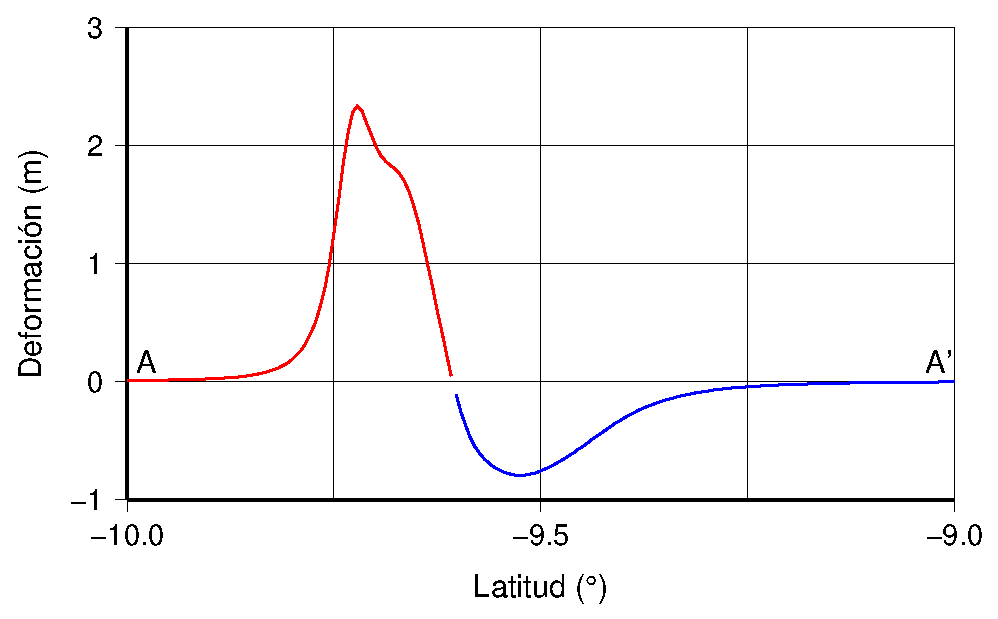
\includegraphics[scale=0.64]{figura.eps}}
	\caption{Ejemplo de Figura (en formato eps Encapsulated Post Script).}
	\label{figura1}
\end{figure}

% Ejemplo de Tabla 
\begin{table}
	\centerline{
		\begin{tabular}{l c c c r}
			\toprule
			$N$ & $v_p (km/s)$ & $v_s (km/s)$ & $\rho (g/cm^3)$ & $t (km)$ \\
			\midrule
			1 &  1.50 & 0.00 & 1.02 &  4.2 \\
			2 &  5.66 & 3.23 & 2.60 &  2.0 \\
			3 &  5.92 & 3.38 & 2.60 &  8.0 \\
			4 &  6.20 & 3.54 & 2.90 & 12.0 \\
			5 &  6.44 & 3.68 & 3.38 &  8.0 \\
			6 &  6.87 & 3.92 & 3.38 & 20.0 \\
			7 &  7.92 & 4.52 & 3.37 &  0.0 \\
			\bottomrule
	\end{tabular}}
	\smallskip
	\caption{Modelo de Tabla.}
	\label{tabla1}
\end{table}

\section{Resultados y Discusión}
Ecuacion con una integral:
\begin{equation}
\label{eq:3}
M_0=\frac{4\pi\rho v^3 R_t}{R_{\theta \varphi}}\int_{\tau_1}^{\tau_2} s(t)\,dt \   
\end{equation}

\begin{equation}
\label{eq:4}
A=\int_{a}^{b} f(x)\,dx \   
\end{equation}

La ecuación de Schrodinger $\hat{H} \Psi = E \Psi $ es una ecuación de
valores propios:

\begin{equation}
i\hbar\frac{\partial}{\partial t}\left|\Psi(t)\right>=H\left|\Psi(t)\right>
\end{equation}

\section{Conclusiones}
Aqui van las conclusiones

De acuerdo a la Figura \ref{figura1}, los valores maximo y minimo son 2.5 y -0.8.

\section*{Agradecimientos}
Aqui van los agradecimientos. Primero se agradece a las personas y luego a las instituciones.

\begin{thebibliography}{99}
\bibitem{1} N. Apellido. Titulo del artículo. Rev. Inv. Fis., \textbf{21}(1), 18-26 (2018).

\bibitem{2} H. Benny y J. Pérez. \emph{Título de Libro}. Editorial San Marcos, Lima (2018).

\bibitem{3} Y. Okada. Internal deformation in a half space. Bull. Seismol. Soc.Am. \textbf{82}(2) 1018-1040 (1992).

\bibitem{4} M. Bazant and J. Bush. Beyond six feet: A guideline to limit indoor airborne transmission of COVID-19, doi: \url{http://doi.org/10.1101/2020.08.26.20182824}.

\bibitem{5} M. Kikuchi y H. Kanamori. \emph{Notes on Teleseismic Body-Wave Inversion Program} \url{http://www.eri.u-tokyo.ac.jp/ETAL/KIKUCHI} (2003).

\bibitem{6} H. Pulker. \emph{Coatings On Glass}. Elsevier Science, 2nd edition. Amsterdam (1999).

\end{thebibliography}

\end{document}
